
\chapter{Cross-validation for unsupervised learning}\label{C:cvul}

The problem unsupervised learning (UL) tries to to address is this: given some
data, describe its distribution. Many estimation problems can be cast as
unsupervised learning, including mean estimation, density estimation, and
linear regression. However, more commonly unsupervised learning refers to
either clustering or manifold learning. A canonical example is principal
component analysis (PCA). In PCA, we are given some high-dimensional data,
and we look for a lower-dimensional subspace that explains most of the
variation in the data. The lower-dimensional subspace describes the
distribution of the data. In clustering, the estimated cluster centers give us
information about the distribution of the data. The output of every UL method
is a summary statistic designed to convey information about the process which
generated the data.

Many UL problems involve model selection. For example, in principal component
analysis we need to choose how many components to keep. For clustering, we
need to choose the number of clusters in the data. Many manifold learning
techniques require choosing bandwidth or a kernel. Often in these contexts,
model-selection is done in an ad-hoc manner. Rules of thumb and manual
inspection guide most choices for how many components to keep, how many
clusters are present, and what is an appropriate kernel. Such informal
selection rules can be problematic when different researches come to different
conclusions about what the right model is. Moreover, even when there is an
obvious ``natural'' model to human eyes, it may be hard to pick out in
computer-automated analysis. For objectivity and efficiency, it is desirable to have a well-specified automatic model selection procedure.

For concreteness, in this chapter we focus on principal components, though
many of the ideas generalize to other methods. We suppose that the data,
$\mX$, is an $n \times p$ matrix generated according to the signal-plus-noise
model $\mX = \sqrt{n} \mU \mD \mV^\trans + \mE$. We consider the first term to
be the ``signal'' matrix, and the second term to be ``noise''. Often the
signal term is a low-rank product. Our goal is to estimate this term as
best as possible by truncating the singular value decomposition (SVD) of
$\mX$. Here ``best'' means with respect to the metrics introduced in
Chapter~\ref{C:intrinsic-rank}. We are interested in the model selection
problem where each model is defined by the number of terms we keep from the
SVD of $\mX$.

We would like our model selection procedure to be non-parametric, if possible.
To work in a variety of contexts, the selection procedure cannot assume
Gaussianity or independence across samples. We would like the procedure to be
driven by the empirical distribution of the data. Cross-validation (CV) is a
popular approach to model selection that generally meets these criteria.
Therefore, we seek to adapt CV to our purposes.

CV prescribes dividing a data set into a ``test'' set and a
``train'' set, fitting a model to the training set, and then evaluating the
model's performance on the test set. We repeat the fit/evaluate procedure
multiple times over different test/train partitions, and then average over all
replicates. Traditionally, the partitions are chosen so that each datum occurs
in exactly one test set. As for terminology, for a particular replicate the
test set is commonly referred to as the held-out or left-out set, and likewise
the train set is often called the held-in or left-in set.

Most often, cross-validation is applied in supervised contexts. In supervised
learning (SL) the data consists of a sequence of $(\vx, \vy)$
predictor-response pairs. Broadly construed, the goal of supervised learning
is to describe the conditional distribution of $\vy$ given $\vx$. This is
usually for prediction or classification.  In the supervised context, for a 
particular CV replicate there are four parts of data:
\[
    \left(
    \begin{matrix}
        \mX_\train & \mY_\train \\
        \mX_\test  & \mY_\test
    \end{matrix}
    \right).
\]
Implicit in the description of cross-validation is that the replicates use
$\mX_\test$ to predict $\mY_\test$. So, the held-in data looks like
\[
    \left(
    \begin{matrix}
        \mX_\train & \mY_\train \\
        \mX_\test  & \missing
    \end{matrix}
    \right).
\]
We extrapolate from $\mX_\test$ to predict $\mY_\test$.

It is not immediately obvious how to apply cross-validation to unsupervised
learning.  In unsupervised learning there is no $\mY$; we instead have the 
two-way partition
\[
    \left(
    \begin{matrix}
        \mX_\train \\
        \mX_\test
    \end{matrix}
    \right).
\]
There is nothing to predict!  Renaming $\mX$ to $\mY$ does not make the
problem any better, for then the division becomes:
\[
    \left(
    \begin{matrix}
        \mY_\train \\
        \mY_\test
    \end{matrix}
    \right),
\]
with hold-in
\[
    \left(
    \begin{matrix}
        \mY_\train \\
        \missing
    \end{matrix}
    \right).
\]
Now, there is nothing to extrapolate from to predict $\mY_\test$!  For 
cross-validation to work in unsupervised learning, we need to consider
more general hold-outs.

We look at two different types of hold-outs in this chapter. The first, due to
Wold, is ``speckled'': we leave out random elements of the matrix $\mX$ and
use a missing data algorithm like expectation-maximization (EM) for
prediction. The second type of hold-out is ``blocked''. This type, due to
Gabriel, randomly partitions the columns of $\mX$ into ``predictor'' and
``response'' sets and then performs the SL version of cross-validation.

\section{Assumptions, and notation}\label{S:ucv-assumptions-notation}

We will generally assume we have data $\mX \in \reals^{n \times p}$
generated according to the latent factor model 
\[
    \mX = \sqrt{n} \, \mU \mD \mV^\trans + \mE.
\]
Here, $\mU \in \reals^{n \times k_0}$, $\mV \in \reals^{n \times k_0}$, and
$\mD = \diag( d_1, d_2, \ldots, d_{k_0} )$, with $\mU^\trans \mU = \mI_{k_0}$
$\mV^\trans \mV = \mI_{k_0}$, and $d_1 \geq d_2 \geq \cdots \geq d_{k_0} > 0$. We call $\sqrt{n} \, \mU \mD \mV^\trans$ the
signal part and $\mE$ the noise part. In the spirit of data-driven analysis,
we avoid putting distributional assumptions on $\mU$, $\mD$, $\mV$, and $\mE$.
This makes the terms unidentifiable.  While this indeterminacy can (and 
should!) bother some readers, for now we will plod on.

We denote the SVD of $\mX$ by
\[
    \mX = \sqrt{n} \, \mhU \mhD \mhV^\trans, 
\]
with $\mhU \in \reals^{n \times n \wedge p}$, $\mhV \in \reals^{p \times n
\wedge p}$, and $\mhD = \diag( \hd_1, \hd_2, \ldots, \hd_{n \wedge p})$. Here,
$\mhU^\trans \mhU = \mhV^\trans \mhV = \mI_{n \wedge p}$ and the singular
values are ordered
\(
    \hd_1 \geq \hd_2 \geq \cdots \geq \hd_{n \wedge p} \geq 0.
\)
We set $\mhD(k) = \diag( \hd_1, \hd_2, \ldots, \hd_k, 0, \ldots, 0) \in \reals^{n \wedge p \times n \wedge p}$ so that
\[
    \mhX(k) = \sqrt{n} \, \mhU \mhD(k) \mhV^\trans
\]
is the SVD of $\mX$ truncated to $k$ terms.  Similarly, we define $\mhU(k) \in 
\reals^{n \times k}$ and $\mhV(k) \in \reals^{p \times k}$ to be the first $k$ 
rows of $\mhU$ and $\mhV$, respectively.

We focus on estimating the squared Frobenius model error
\[
    \ME(k) = \| \sqrt{n} \, \mU \mD \mV^\trans - \mhX(k) \|_\Frob^2
\]
or its minimum,
\[
    k^\ast_{\ME} = \argmin_k \ME(k).
\]  
Here, $\| \cdot \|_\Frob^2$ is the sum of squares of the elements.

Another kind of error relevant to cross-validation is \emph{prediction error}.  We let $\mE'$ be a matrix independent of $\mE$ but having the same distribution conditionally on $\mU$, $\mD$, and $\mV^\trans$.  We set 
\[
    \mX' = \sqrt{n} \, \mU \mD \mV^\trans + \mE'
\]
and define the prediction error
\[
    \PE(k) = \E \| \mX' - \mhX(k) \|_\Frob^2.
\]
Likewise, we set
\[
    k^\ast_{\PE} = \argmin_k \PE(k).
\]
If $\mE$ is independent of $\mU$, $\mD$, and $\mV$, then
\begin{align*}
    \PE(k) 
        &= \E\| \sqrt{n} \, \mU \mD \mV^\trans - \mhX(k) + \mE' \|_\Frob^2 \\
    \begin{split}
        &= \E\| \sqrt{n} \, \mU \mD \mV^\trans - \mhX(k) \| \\
           &\qquad\qquad+ 
           2 \, 
           \E \left[
               \tr \left( 
                   \big( \sqrt{n} \, \mU \mD \mV^\trans - \mhX(k) \big)^\trans 
                   \mE'
               \right)
           \right]
           +
           \E\| \mE' \|_\Frob^2 
    \end{split} \\
        &= \E\big[\ME(k)\big] + \E \| \mE \|_\Frob^2.
\end{align*}
The prediction error is thus equal to the sum of the expected model error
and an irreducible error term.

Finally, we should note that our definitions of prediction error and model
error are motivated by the definitions given by
Breiman~\cite{breiman1992little} for cross-validating linear regression.


\section{Cross validation strategies}

In this section we describe the various hold-out strategies for getting a
cross-validation estimate of $\PE(k)$. It is possible to get an estimate of
$\ME(k)$ from the estimate of $\PE(k)$ by subtracting an estimate of the
irreducible error. For now, though, we choose to focus just on estimating
$\PE(k)$.

For performing $K$-fold cross-validation on the matrix $\mX$, we partition its
elements into $K$ hold-out sets. For each of $K$ replicates and for each value
of the rank, $k$, we leave out one of the hold-out sets, fit a $k$-term SVD to
the left-in set, and evaluate its performance on the left-out set. We thus
need to describe the hold-out set, how to fit an SVD to the left-in data, and
how to make a prediction of the left-out data. After a brief discussion of why
the usual (naive) way of doing hold-outs won't work, we survey both speckled
hold-outs (Wold-style), as well as block hold-outs (Gabriel-style).

\subsection{Naive hold-outs}

The ordinary hold-out strategy will not work for estimating prediction error.  Suppose we leave out a subset of the rows of $\mX$.  After
permutation, the rows of $\mX$ are partitioned as
\(
    \left(
    \begin{matrix}
        \mX_1 \\
        \mX_2
    \end{matrix}
    \right),
\)
where $\mX_1 \in \reals^{n_1 \times p}$ and $\mX_2 \in \reals^{n_2 \times p}$,
and $n_1 + n_2 = n$.  The only plausible prediction of $\mX_2$ based on truncating the SVD of $\mX_1$ is the following:
\begin{enumerate}
    \item Let $\mX_1 = \sqrt{n} \, \mhU_1 \mhD_1 \mhV_1^\trans$ be the SVD of
        $\mX_1$, with 
        \(
            \mhD_1 
                = 
                \diag( 
                    \hd_1^{(1)}, 
                    \hd_2^{(1)}, 
                    \ldots, 
                    \hd_{n_1 \wedge p}^{(1)}
                ).
        \)
    \item Let 
        \(
            \mhD_1(k)
                =
                \diag(
                    \hd_1^{(1)}\!\!\!, \,
                    \hd_2^{(1)}\!\!\!, 
                    \ldots, 
                    \hd_k^{(1)}\!\!\!, \,
                    0,
                    \ldots,
                    0
                )
        \)
        so that
        $\mhX_1(k) \equiv \sqrt{n} \, \mhU_1 \mhD_1(k) \mhV_1^\trans$ is
        the SVD of $\mX_1$ truncated to $k$ terms.  Similarly, denote
        by $\mhV_1(k) \in \reals^{p \times k}$ the first $k$ columns of
        $\mhV_1$.
    \item Let $(^+)$ denote pseudo-inverse and predict the held out rows as
        \(
            \mhX_2(k) 
                = 
                    \mX_2 \,
                    \mhX_1(k)^\trans
                    \big(
                        \mhX_1(k) \mhX_1(k)^\trans
                    \big)^{+}
                    \mhX_1(k)
                =
                    \mX_2 \, \mhV_1(k) \mhV_1(k)^\trans.
        \)
\end{enumerate}
The problem with this procedure is that $\| \mX_2 - \mhX_2(k) \|_\Frob^2$ 
decreases with $k$ regardless of the true model for $\mX$.  So, it cannot
possibly give us a good estimate of the error from truncating the full
SVD of $\mX$.

A similar situation arrises if we leave out only a subset of the columns of
$\mX$.  To get a reasonable cross-validation estimate, it is therefore 
necessary to consider more-general hold-out sets.

\subsection{Wold hold-outs}

A Wold-style speckled leave-out is perhaps the most obvious attempt at a a
more general hold-out. We leave out a subset of the elements of the $\mX$, then
use the left-in elements to predict the rest.

First we need to introduce some more notation. Let $\mathcal{I}$ denote the
set of indices of the elements of $\mX$, so that $\mathcal{I} = \{ (i,j) : 1
\leq i \leq n, 1 \leq j \leq p \}$. For a subset $I \subset \mathcal{I}$, let
$\bar I$ denote its complement $\mathcal{I} \setminus I$. We use the symbol
$\missing$ to denote a missing value, and let 
\(
    \reals_\missing = \reals \cup \{ \missing \}.
\)
For $I \subset \mathcal{I}$, we define the matrix $\mX_I \in
\reals_\missing^{n \times p}$ with elements
\[
    X_{I,ij}
    =
    \begin{cases}
        X_{ij}     &\text{if $(i,j) \in I$,} \\
        \missing   &\text{otherwise.}
    \end{cases}
\]
Similarly $\mX_{\bar I}$, has elements
\[
    X_{\bar I,ij}
    =
    \begin{cases}
        X_{ij}     &\text{if $(i,j) \notin I$,} \\
        \missing   &\text{otherwise.}
    \end{cases}
\]
Finally, for $\mA \in \reals_\missing^{n \times p}$, we define
\[
    \| \mA \|_{\Frob,I}^2
        =
        \sum_{(i,j) \in I} A_{ij}^2.
\]
This notation allows us to describe matrices with missing entries.

A Wold-style speckled hold-out is a random subset $I \subset \mathcal{I}$.  The 
held-in data is the matrix $\mX_{\bar I}$ and the held-out data is the matrix 
$\mX_I$.  We use a missing value SVD algorithm to fit a $k$-term SVD to 
$\mX_{\bar I}$.  This gives us an approximation $\mU_k \mD_k \mV_k^\trans$, 
where $\mU_k \in \reals^{n \times k}$ and $\mV_k \in \reals^{p \times k}$ have 
orthonormal columns and $\mD \in \reals^{k \times k}$ is diagonal.  We 
evaluate the SVD on the held-out set by 
\(
    \| \mU_k \mD_k \mV_k^\trans - \mX_I \|_{\Frob,I}^2.
\)
Aside from the algorithm for getting $\mU_k \mD_k \mV_k^\trans$ from 
$\mX_{\bar I}$, this is a full description of the CV replicate.

When Wold introduced this form of hold-out in 1978~\cite{wold1978cross}, he
suggested using an algorithm called nonlinear iterative partial least squares
(NIPALS) to fit an SVD to the held-in data. This algorithm, attributed to
Fisher~\cite{fisher1923scv}, Wold and Lyttkens~\cite{wold1969nonlinear} never
seems to have gained much prominence. We suggest instead using an
expectation-maximization (EM) as is consistent with current mainstream
practice in Statistics. Either way, there are some subtle issues in taking the
SVD of a matrix with missing values. We explore these issues further in
Section~\ref{S:missing-values-svds}, and present a complete algorithm for
estimating the factors $\mU_k \mD_k \mV_k^\trans$.

\subsection{Gabriel hold-outs}

A Gabriel-style hold-out works by transforming the unsupervised learning
problem into a supervised one. We take a subset of the columns of $\mX$ and
denote them as the \emph{response} columns; the rest are denoted
\emph{predictor} columns. Then we take a subset of the rows and consider them
as \emph{test} rows; the rest are \emph{train} rows. This partitions the
elements of $\mX$ into four blocks. With permutation matrices $\mP$ and $\mQ$,
we can write
\[
    \mP^\trans \mX \mQ
        =
        \left(
        \begin{matrix}
           \mX_{11} & \mX_{12} \\
           \mX_{21} & \mX_{22}
        \end{matrix}
        \right).
\]
Here, $\mX_{11}$ consists of the train-predictor block, $\mX_{12}$ is the train-response block, $\mX_{21}$ is the test-predictor block, and $\mX_{22}$ is the test-response block.  It is beneficial to think of the blocks as
\[
    \left(
    \begin{matrix}
       \mX_{11} & \mX_{12} \\
       \mX_{21} & \mX_{22}
    \end{matrix}
    \right)
        =
        \left(
        \begin{matrix}
           \mX_\train & \mY_\train \\
           \mX_\test  & \mY_\test 
        \end{matrix}
        \right).
\]
A Gabriel-style replicate has hold-in
\[
\left(
    \begin{matrix}
       \mX_{11} & \mX_{12} \\
       \mX_{21} & \missing
    \end{matrix}
    \right)
\]
and hold-out $\mX_{22}$.

To fit a model to the hold-in set, we take the SVD of $\mX_{11}$ and fit a 
regression function from the predictor columns to the response columns.  
Normally, the regression is ordinary least squares regression from the 
principal component loadings to the response columns.  Then, to evaluate the 
function on the hold-out set, we apply the estimated regression function to 
$\mX_{21}$ to get a prediction $\mhX_{22}$.

In precise terms, suppose that there are $p_1$ predictor columns, $p_2$ response columns, $n_1$ train rows, and $n_2$ test rows.  Then $\mX_{11} \in \reals^{n_1 \times p_1}$ and $\mX_{22} \in \reals^{n_2 \times p_2}$ with
$p_1 + p_2 = p$ and $n_1 + n_2 = n$.  First we fit an SVD to the train-predictor block 
\[
    \mX_{11} = \sqrt{n} \, \mhU_1 \mhD_1 \mhV_1^\trans.  
\]    
Then, we truncate the SVD to $k$ terms as 
$\sqrt{n} \, \mhU_1(k) \mhD_1(k) \mhV_1^\trans(k)$ in the same way as is discussed 
in Section~\ref{S:ucv-assumptions-notation}.  This defines a projection 
$\mhV_1(k)$ and principal component scores 
\[
    \mhZ_1(k) = \mX_{11} \mhV_1(k) = \sqrt{n} \, \mhU_1(k) \mhD_1(k).
\]
Similarly, we can get the principal components scores for the test-predictor block as
\[
    \mhZ_2(k) = \mX_{21} \mhV_1(k).
\]
Next, we model the response columns as linear functions of the principal component scores.  We fit the model
\(
    \mX_{12} = \mhZ_1(k) \mB
\)
with
\[
    \mhB 
        =
        \big( \mhZ_1(k)^\trans \mhZ_1(k) \big)^{+} \mhZ_1(k)^\trans \mX_{12}
        =
        \frac{1}{\sqrt{n}} \,
        \mhD_1(k)^{+} \, \mhU_1(k)^\trans \mX_{12}.
\]
Finally, we apply the model the the test rows to get a prediction for the test-response block
\[
    \mhX_{22}
        =
        \mhZ_2(k) \mhB
        =
        \mX_{21} 
        \left(
            \frac{1}{\sqrt{n}} \,
            \mhV_1(k) \mhD_1(k)^{+} \, \mhU_1(k)^\trans 
        \right)
        \mX_{12}.
\]
This gives a complete description of the CV replicate.

We can get some intuition for why Gabriel-style replicates work by expressing 
the latent factor decomposition $\mX = \sqrt{n} \,\mU \mD \mV^\trans + \mE$ in 
block form.  We let
\(
    \mP
    =
    \left(
    \begin{matrix}
        \mP_1 &
        \mP_2
    \end{matrix}
    \right)
\)
and
\(
    \mQ
    =
    \left(
    \begin{matrix}
        \mQ_1 &
        \mQ_2
    \end{matrix}
    \right)
\)
be the block-decompositions of the row and column permutations so that
$\mX_{ij} = \mP_i^\trans \mX \mQ_j$.  We define $\mU_i = \mP_i^\trans \mU$,
$\mV_j = \mQ_j^\trans \mV$, and $\mE_{ij} = \mP_i^\trans \mE \mQ_j$ so that
\begin{align*}
    \mP^\trans \mX \mQ
        &=
            \left(
            \begin{matrix}
                \mP_1^\trans \\
                \mP_2^\trans
            \end{matrix}
            \right)
            \left(
                \sqrt{n} \, \mU \mD \mV^\trans + \mE
            \right)
            \left(
            \begin{matrix}
                \mQ_1 & \mQ_2
            \end{matrix}
            \right) \\
        &=
            \sqrt{n}
            \left(
            \begin{matrix}
                \mU_1 \mD \mV_1^\trans
                    & \mU_1 \mD \mV_2^\trans  \\
                \mU_2 \mD \mV_1^\trans
                    & \mU_2 \mD \mV_2^\trans
            \end{matrix}
            \right)
            +
            \left(
            \begin{matrix}
                \mE_{11} & \mE_{12} \\
                \mE_{21} & \mE_{22}
            \end{matrix}
            \right).
\end{align*}
Thus, all four blocks have the same low-rank structure.  If the noise is small 
then $\mX_{22} \approx \sqrt{n} \, \mU_2 \mD \mV_2^\trans$ and
\[
    \mhX_{22} 
        \approx 
            \sqrt{n} \,
                \mU_2 \mD 
                \big( \mV_1^\trans \mhV_1(k) \big) \,
                \mhD(k)^{+} \,
                \big( \mhU_1(k)^\trans \mU_1 \big) \,
                \mD \mV_2^\trans
\]
If the noise is exactly zero, $k = k_0$, and $\rank(\mX_{22}) = \rank(\mX)$, 
then Owen and Perry~\cite{owen2009bi} show that $\mhX_{22} = \mX_{22}$.  For 
other types of noise, the next chapter proves a more general consistency 
result.

\subsection{Rotated cross-validation}\label{SS:rotated-cv}

When the underlying signal $\mU \mD \mV^\trans$ is sparse, it's possible that we will miss it in the training set.  For example, if 
\(
    \mU 
    =
    \left(
    \begin{matrix}
        1 & 0 & 0 & 0
    \end{matrix}
    \right)^\trans
\)
and
\(
    \mV
    =
    \left(
    \begin{matrix}
        1 & 0 & 0 & 0 & 0
    \end{matrix}
    \right)^\trans
\),
then
\[
    \mU \mD \mV^\trans
    =
    \left(
    \begin{matrix}
        d_{1} & 0 & 0 & 0 & 0 \\
        0     & 0 & 0 & 0 & 0 \\
        0     & 0 & 0 & 0 & 0 \\
        0     & 0 & 0 & 0 & 0 
    \end{matrix}
    \right).
\]
Either the test set will observe this factor, or the train set, but not both.  Only the set that contains $X_{11}$ will be affected by the factor.

One way to adjust for sparse factors is to randomly rotate the rows and
columns of $\mX$ before performing the cross-validation. We generate $\mP \in
\reals^{n \times n}$ and $\mQ \in \reals^{p \times p}$, uniformly random
orthogonal matrices, by employing Algorithm~\ref{A:random-steifel}. Then, we
set $\mtX = \mP \mX \mQ^\trans$ and perform ordinary cross-validation on
$\mtX$. Regardless of the factor structure in $\mX$, the signal part of $\mtX$
will be uniformly spread across all elements of the matrix. We call this
procedure \emph{rotated cross-validation}, abbreviated RCV.  

RCV is similar in spirit to the generalized cross-validation (GCV) described
in Craven \& Wahba~\cite{craven1978smoothing} and Golub et
al.~\cite{golub1979generalized}. GCV is an orthogonally-invariant way of
performing leave-one-out cross validation for regression. The difference is
that GCV rotates to a specific non-random configuration of the data that gives
equal weight to all observations in the rotated space, while RCV rotates to a 
random configuration that gives equal weight in expectation.


\section{Missing-value SVDs}\label{S:missing-values-svds}

To perform a Wold-style cross-validation we need to be able to compute the SVD of a matrix with missing entries.  This is a difficult problem.  First of all, the problem is not very well defined.  If $\mA$ is a matrix with missing entries, there are potentially many different ways of factoring $\mA$ as an SVD-like product.  Often, one attempts to force uniqueness by finding the complete matrix $\mA' \in \reals^{n,p}$ of minimum rank such that $A'_{ij} = A_{ij}$ for all non-missing elements of $\mA$.  Even then, $\mA'$ may not be unique.  Take
\[
    \mA
    =
    \left(
    \begin{matrix}
        1        & \missing \\
        \missing & \missing
    \end{matrix}
    \right).
\]
Then
\[
    \left(
    \begin{matrix}
        1 & 0 \\
        0 & 0
    \end{matrix}
    \right),
    \quad
    \left(
    \begin{matrix}
        1 & 1 \\
        0 & 0
    \end{matrix}
    \right),
    \quad
    \left(
    \begin{matrix}
        1 & 0 \\
        1 & 0
    \end{matrix}
    \right),
    \quad
    \text{and}
    \quad
    \left(
    \begin{matrix}
        1 & 1 \\
        1 & 1
    \end{matrix}
    \right)
\]
are all rank-$1$ matrices that agree with $\mA$ on its non-missing entries.  We might discriminate between these by picking the matrix with minimum Frobenius norm.  In this case, the matrix
\[
    \left(
    \begin{matrix}
        1 & \missing \\
        \missing & 1
    \end{matrix}
    \right)
\]
presents an interesting problem.  We can either complete it as
\[
    \left(
    \begin{matrix}
        1 & 1 \\
        1 & 1
    \end{matrix}
    \right)
    \quad
    \text{or}
    \quad
    \left(
    \begin{matrix}
        1 & 0 \\
        0 & 1
    \end{matrix}
    \right).
\]
The first option has rank $1$ and Frobenius norm $2$.  The second option
has higher rank, $2$, but lower Frobenius norm, $\sqrt{2}$.  Which criterion 
is more important?  It it not clear what the ``right'' SVD of $\mA$ is.

We can ameliorate the problem by considering a sequence of SVDs rather than a 
single one.  For each $k = 0, 1, 2, \ldots$, define $\mA_k'$ to the the 
rank-$k$ matrix of minimum Frobenius norm that agrees with $\mA$ on its 
non-missing elements.  If no such matrix exists, let $I \subset \mathcal{I}$ 
be indices of the non-missing elements of $\mA$ and define the candidate
sets
\begin{align*}
    \mathcal{A}_k 
        &= \{ \mA_k \in \reals^{n \times p} : \rank(\mA_k) = k \} \\
    \mathcal{C}_k
        &= \{ \mA_k \in  \mathcal{A}_k 
                : \| \mA - \mA_k \|_{\Frob,I}
                  =
                  \min_{\mB_k \in \mathcal{A}_k} 
                      \| \mA - \mB_k \|_{\Frob,I} \}.
\end{align*}
Lastly, put
\[
    \mA'_k
        = \argmin_{\mA_k \in \mathcal{C}_k}
            \| \mA_k \|_{\Frob,I}.
\]
We then define the rank-$k$ SVD of $\mA$ to be the equal to the SVD of 
$\mA'_k$.  

There are still some problems with these SVDs. First of all, in general there
may be no relationship between $\mA_k'$ and $\mA_{k+1}'$; the two matrices may
be completely different and have completely different SVDs. We lose the
nesting property of ordinary SVDs, where the rank-$k$ SVD is contained in the
rank $k+1$ SVD. Secondly, although it seems plausible, we do not have any
guarantees that $\mA_k'$ is unique. Situations may arise where two different
rank-$k$ matrices have the same norms and the same residual norms on the
non-missing elements of $\mA$. Finally, finding $\mA'_k$ is a non-convex
problem. The function $\| \mA - \mA_k \|_{\Frob,I}$ can have more than one
local maximum.  We need to be aware of these deficiencies.

Rather than get too deep into the $\reals_\ast$-SVD rabbit hole, we choose
instead to live with an approximation. We acknowledge that computing the best
rank-$k$ approximation as defined above is computationally infeasible for
large $n$ and $p$. Instead of proving theorems about the global optimum, we
focus on an algorithm for computing a local solution.

We use an EM-algorithm to estimate $\mA'_k$. The inputs to the algorithm are
$k$, a non-negative integer rank, and $\mA \in \reals_\missing^{n \times p}$,
a matrix with missing values. The output is $\mA_k'$, a rank-$k$ approximation
of $\mA$. The algorithm proceeds by iteratively estimating the missing values
of $\mA$ by the values from the first $k$ terms of the SVD of the completed
matrix. We give detailed pseudocode for the procedure as
Algorithm~\ref{A:em-svd}. This is essentially the same algorithm as the
SVDimpute algroithm given in Troyanksaya et al.~\cite{troyanskaya2001missing},
except that we use a different convergence criterion. SVDimpute stops when
successive estimates of the missing values of $\mA$ differ by less than ``the
empirically determined threshold of $0.01$.'' We instead stop when relative
difference of the residual sum of squares (RSS) between the non-missing
entries and the rank-$k$ SVD is small (usually $1.0 \times 10^{-4}$ or less).
Our reason for using a different convergence rule is that the analysis of the
EM algorithm in Dempster et al.~\cite{dempster1977maximum} shows that the RSS
decreases with each iteration, but makes no assurances about the missing
values converging. Regardless of which convergence criterion is used, the
algorithm is very easy to implement.

\begin{algorithm}
    \caption{Rank-$k$ SVD approximation with missing values}\label{A:em-svd}
    
    \begin{enumerate}
        \item Let $I = \{ (i,j) : A_{ij} \neq \missing \}$.
        \item For $1 \leq j \leq p$ let $\mu_j$ be the mean of the
            non-missing values in column $j$ of $\mA$, or $0$ if all of
            the entries in column $j$ are missing.
        \item Define $\mA^{(0)} \in \reals^{n \times p}$ by
            \[
                A^{(0)}_{ij}
                    =
                    \begin{cases}
                        A_{ij} &\text{if $(i,j) \in I$,} \\
                        \mu_j  &\text{otherwise.}
                    \end{cases}
            \]
        \item Initialize the iteration count $N \gets 0$.
        \item (\textsc{M-Step}) \label{em-svd-m-step} Let 
            \[
                \mA^{(N)} = 
                    \sum_{i=1}^{n \wedge p}
                        d^{(N)}_i \vu^{(N)}_i \vv^{(N)\trans}_i
            \]
            be the SVD of $\mA^{(N)}$ and let $\mA'^{(N)}_k$ be the SVD 
            truncated to $k$ terms, so that
            \[
                \mA'^{(N)}_k 
                    = 
                        \sum_{i=1}^{k}
                            d^{(N)}_i \vu^{(N)}_i \vv^{(N)\trans}_i.
            \]
        \item (\textsc{E-Step}) Define $\mA^{(N+1)} \in \reals^{n \times p}$ 
            as
            \[
                A^{(N+1)}_{ij}
                    =
                    \begin{cases}
                        A_{ij}           &\text{if $(i,j) \in I$,} \\
                        A'^{(N)}_{k,ij}  &\text{otherwise.}
                    \end{cases}
            \]
        \item Set 
            \[
                \text{RSS}^{(N)} = \| \mA - \mA'^{(N)}_k \|^2_{\Frob,I}.
            \]
            If $|\text{RSS}^{(N)} - \text{RSS}^{(N-1)}|$ is small, declare 
            convergence and output $\mA'^{(N)}_k$ as $\mA'_k$.  
            Otherwise, increment $N \gets N + 1$ and go to
            Step~\ref{em-svd-m-step}.
    \end{enumerate}
\end{algorithm}

\clearpage

\section{Simulations}

We performed two sets of simulations to gauge the performance of Gabriel- and Wold-style cross-validation.  In the first set of simulations, we compare estimated prediction error with true prediction error.  In the second set, we evaluate the methods' abilities to estimate $k_{\PE}^\ast$, the optimal rank.

Each simulation generates a data matrix $\mX$ as 
\(
    \mX = \sqrt{n} \mU \mD \mV^\trans + \mE.
\)
We fix the dimensions and number of generating signals as $n = 100$, $p = 50$,
and $k_0 = 6$.  For ``weak'' factors we set 
\(
    \mD 
    = 
    \mD_\text{weak}
    =
    \diag \left(
        10, 9, 8, 7, 6, 5
    \right)
\)
and for ``strong'' factors, we set
\(
    \mD
    =
    \mD_\text{strong}
    =
    \sqrt{n} \mD_\text{weak}.
\)
We generate $\mU$, $\mV$, and $\mE$ independently of each other.  To avoid 
ambiguity in what constitutes ``signal'' and what constitutes ``noise'', we 
ensure that the elements of $\mE$ are uncorrelated with each other.

We consider two types of factors.  For ``Gaussian'' factors, we put the elements of $\mU$ distributed \iid with
$U_{11} \sim \Normal\big( 0, \, \frac{1}{n} \big)$ and the elements of
$\mV$ \iid with $V_{11} \sim \Normal\big( 0, \, \frac{1}{p} \big)$, also independent of $\mU$.  For ``Sparse'' factors we use sparsity parameter $s = 10\%$ and set
\[
    \Prob\{ U_{11} = 0 \} = 1 - s,
\]
\[
    \Prob\Big\{ U_{11} = -\frac{1}{\sqrt{s \, n}} \Big\}
    =
    \Prob\Big\{ U_{11} = +\frac{1}{\sqrt{s \, n}} \Big\}    
    = 
    \frac{s}{2}.
\]
Similarly, we put
\[
    \Prob\{ V_{11} = 0 \} = 1 - s,
\]
\[
    \Prob\Big\{ V_{11} = -\frac{1}{\sqrt{s \, p}} \Big\}
    =
    \Prob\Big\{ V_{11} = +\frac{1}{\sqrt{s \, p}} \Big\}    
    = 
    \frac{s}{2}.
\]
The scalings in both cases are chosen so that $\E [\mU^\trans \mU] = \E 
[\mV^\trans \mV] = \mI_{k_0}$.  Gaussian factors are uniformly spread out in the observations and variables, while sparse factors are only observable in a small percentage of the matrix entries (about $1\%$).

We use three types of noise.  For ``white'' noise, we generate the elements of $\mE$ \iid with $E_{11} \sim \Normal\left( 0, \, 1\right)$.  For ``heavy'' noise, we use \iid elements with $E_{11} \sim \sigma_\nu^{-1} \, t_\nu$, and
$\nu = 3$.  Here $t_\nu$ is a $t$ random variable with $\nu$ degrees of freedom, and $\sigma_\nu = \sqrt{\nu/(\nu-2)}$ is chosen so that 
$\E [ E_{11}^2 ] = 1$.  Heavy noise is so-called because it has a heavy tail.  Lastly, for ``colored'' noise, we first generate
$\sigma^2_1, \ldots, \sigma^2_n \sim \text{Inverse-$\chi^2$}(\nu_1)$ and
$\tau^2_1, \ldots, \tau^2_p \sim \text{Inverse-$\chi^2$}(\nu_2)$ independently, with $\nu_1 = \nu_2 = 3$.  Then we generate the elements of $\mE$ independently as
\(
    E_{ij} \sim 
        c_{\nu_1, \nu_2}^{-1} \, \cdot \Normal( 0, \, \sigma^2_i + \tau^2_j),
\)
where
\(
    c_{\nu_1, \nu_2}
        =
        \sqrt{1/(\nu_1 - 2) + 1/(\nu_2 - 2)}
\).
Again, $c_{\nu_1, \nu_2}$ is chosen so that $\E [E_{ij}^2] = 1$.  Colored 
noise simulates heteroscedasticity.  All three types of noise are plausible 
for real-world data.


\subsection{Prediction error estimation}

Our goal with the first simulation was to get intuition for the behavior of
Gabriel- and Wold-style cross validation as prediction error estimators. We
generated random data of the form $\mX = \sqrt{n} \mU \mD \mV^\trans + \mE$,
described above. With $\mhX(k)$ being the SVD of $\mX$ truncated to $k$ terms,
the (normalized) true prediction error is given by
\[ 
    \PE(k) = \| \sqrt{n} \mU \mD \mV^\trans - \mhX(k) \|_\Frob^2 + 1. 
\] 
Cross-validation gives us an estimate $\widehat{\PE}(k)$ of the prediction 
error curve.  We wanted to see how $\widehat{\PE}(k)$ compares to $\PE(k)$.

Figures~\ref{F:cvsvd-pe-strong}~and~\ref{F:cvsvd-pe-weak} show the true and
estimated prediction error curves from $(2,2)$-fold Gabriel CV and $5$-fold
Wold CV, along with their RCV variants. The plots only show one set of curves
for each factor and noise instance, but other replicates showed similar
behavior.  

For most of the simulations, the cross-validation estimates of prediction
error are generally conservative. The only exception is with weak factors and
colored noise, perhaps because of the ambiguity in what constitutes ``signal''
and what constitutes ``noise'' in this simulation. This global upward bias
agrees with previous studies of cross-validation 
(e.g.~\cite{breiman1992little} and \cite{breiman1992submodel}).  The RCV versions of the methods generally brought down the bias.  Some authors have observed a downward bias at the minimizer of $\widehat{\PE}(k)$ for ordinary cross-validation (\cite{breiman1984cart}, \cite{tibshirani2009}).  This bias does not appear to be present here.

A striking difference between Wold- and Gabriel-style CV is their behavior for $k$ greater than $k^\ast_{\PE}$.  Gabriel-style CV does a better job at estimating the true $\PE(k)$, which is relatively flat.  Wold-style CV, on the other hand, increases steeply for $k$ past the minimizer.  Since estimating $\PE(k)$ past its minimizer is generally of very little interest, the Wold-style CV behavior is more desirable.

\begin{figure}[ht]
    \centering
    \begin{minipage}{0.49\textwidth}
        \begin{center}
            \includegraphics[scale=0.66]{cvsvd-strong-gauss}
        \end{center}
    \end{minipage}
    \begin{minipage}{0.49\textwidth}
        \begin{center}
            \includegraphics[scale=0.66]{cvsvd-strong-sparse}
        \end{center}
    \end{minipage}
    \caption{
        \captiontitle{Cross-validation with strong factors}
        Estimated prediction error curves for Gabriel- and Wold-style
        cross-validation, both original and rotated (RCV) versions, with
        strong factors in the data.  
        The true prediction error is shown in black, the CV curves are red, 
        and the RCV curves are blue.  Error bars give are computed from the 
        CV replicates.  Despite their upward bias, the methods do
        well at estimating $\PE(k)$ for $k \leq k^\ast_{\PE}$.
    }\label{F:cvsvd-pe-strong}
\end{figure}


\begin{figure}[ht]
    \centering
    \begin{minipage}{0.49\textwidth}
        \begin{center}
            \includegraphics[scale=0.66]{cvsvd-weak-gauss}
        \end{center}
    \end{minipage}
    \begin{minipage}{0.49\textwidth}
        \begin{center}
            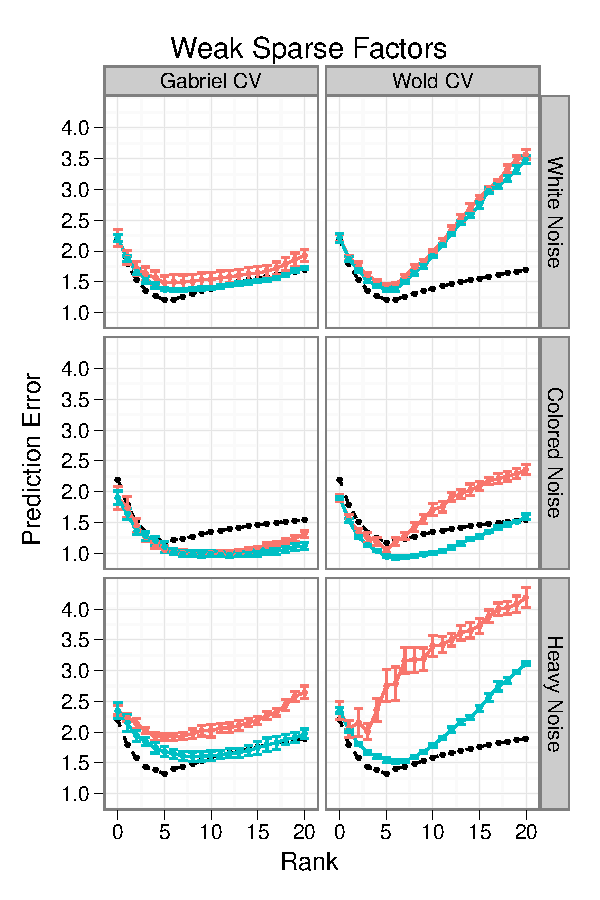
\includegraphics[scale=0.66]{cvsvd-weak-sparse}
        \end{center}
    \end{minipage}
    \caption{
        \captiontitle{Cross-validation with weak factors}
        Estimated prediction error curves for Gabriel- and Wold-style
        cross-validation, both original and rotated (RCV) versions, with
        weak factors in the data.  As in Figure~\ref{F:cvsvd-pe-strong} the
        true prediction error is shown in black, the CV curves are red, and
        the RCV curves are blue.  Error bars give are computed from the 
        CV replicates.  The methods have a harder time estimating $\PE(k)$
        and its minimizer.
    }\label{F:cvsvd-pe-weak}
\end{figure}

\clearpage 

\subsection{Rank estimation}

In the next simulation, we see how well cross-validation works at estimating
the optimal rank, especially as compared to other rank-selection methods.  We 
generate data in the same manner as before, and record how far off the 
minimizer of $\widehat{\PE}(k)$ is from the minimizer of $\PE(k)$.

We compared the four CV-based rank estimation methods with seven other 
methods.  They are as follows:
\begin{itemize}
    \item AIC: Rao \& Edelman's AIC-based estimator 
        \cite{rao2008sample}.
    \item BIC$_1$, BIC$_2$, and BIC$_3$: Bai \& Ng's BIC-based estimators 
        \cite{bai2002dnf}.
    \item $F$: Faber \& Kowalski's modification of 
        Malinowski's  $F$-test, with a significance level of $0.05$  
        \cite{faber1997critical,malinowski1989statisticalf}.
    \item MDL: Wax \& Kailaith's estimator based on the minimum description 
        length principle
        \cite{wax1985detection} .
    \item UIP: Kritchman \& Nadler's estimator based on Roy's  
        union-intersection principle and their background noise estimator,      
        with a significance level of $0.001$
         \cite{kritchman2008determining,roy1953heuristic}.
\end{itemize}
Kritchman and Nadler \cite{kritchman2008determining} give concise descriptions 
of four of the estimators.  The other estimators, Bai and Ng's BICs, are 
defined as the minimizers of
\begin{align*}
    \text{BIC}_1(k)
        &= \log \| \mX - \mhX(k) \|_\Frob^2
           + k \, \frac{n + p}{n \, p} \log \frac{n \, p}{n + p}, \\
    \text{BIC}_2(k)
        &= \log \| \mX - \mhX(k) \|_\Frob^2
           + k \, \frac{n + p}{n \, p} \log C_{n,p}, \\
    \text{BIC}_3(k)
        &= \log \| \mX - \mhX(k) \|_\Frob^2
           + k \, \frac{\log C_{n,p}^2}{C_{n,p}},
\end{align*}
where $C_{n,p} = \min( \sqrt{n}, \sqrt{p})$.

Tables~\ref{T:rank-est-strong-gauss}--\ref{T:rank-est-weak-sparse} summarize
the results of 100 replicates.  For the strong factors in white noise, almost
all of the methods correctly estimate the true $\PE$-minimizing rank.  When the noise is non-white, Wold-style CV is the clear winner.  For the weak factors in white noise, the AIC, $F$ and UIP methods fare well, and the performance of the cross-validation-based methods is mediocre.  For non-white noise and weak factors, none of the methods perform very well.

\begin{table}
    \tiny
    \centering    
    \begin{tabular}{lrrrrrrrrrrrrrrrr}
        \toprule
        &\multicolumn{15}{c}{\scriptsize{Estimated Rank}} \\
        \cmidrule{2-17}
        \scriptsize{Method}
            & $-7$ & $-6$ & $-5$ & $-4$ & $-3$ & $-2$ & $-1$ 
            & $\phantom{+}0$ 
            & $+1$ & $+2$ & $+3$ & $+4$ & $+5$ & $+6$ & $+7$ & $> 7$ \\
        \midrule
        \\
        &\multicolumn{16}{l}{\scriptsize{\textit{White Noise}}} \\
 CV-Gabriel &  &  &  &  &  &  &  &  99 &  1 &  &  &  &  &  &  & \\ 
 RCV-Gabriel &  &  &  &  &  &  &  &  97 &  2 &  1 &  &  &  &  &  & \\ 
 CV-Wold &  &  &  &  &  &  &  &  100 &  &  &  &  &  &  &  & \\ 
 RCV-Wold &  &  &  &  &  &  &  &  100 &  &  &  &  &  &  &  & \\ 
 AIC &  &  &  &  &  &  &  &  99 &  1 &  &  &  &  &  &  & \\ 
 BIC$_1$ &  &  &  &  &  &  &  &  100 &  &  &  &  &  &  &  & \\ 
 BIC$_2$ &  &  &  &  &  &  &  &  100 &  &  &  &  &  &  &  & \\ 
 BIC$_3$ &  &  &  &  &  &  &  &  100 &  &  &  &  &  &  &  & \\ 
 $F$ &  &  &  &  &  &  &  &  100 &  &  &  &  &  &  &  & \\ 
 MDL &  &  &  &  &  &  &  &  100 &  &  &  &  &  &  &  & \\ 
 UIP &  &  &  &  &  &  &  &  100 &  &  &  &  &  &  &  & \\ 
         \\
        &\multicolumn{16}{l}{\scriptsize{\textit{Colored Noise}}} \\
CV-Gabriel &  &  &  &  &  &  &  &  32 &  42 &  18 &  5 &  2 &  1 &  &  & \\ 
 RCV-Gabriel &  &  &  &  &  &  &  &  6 &  7 &  18 &  13 &  15 &  26 &  9 &  4 &  2\\ 
 CV-Wold &  &  &  &  &  &  &  &  97 &  3 &  &  &  &  &  &  & \\ 
 RCV-Wold &  &  &  &  &  &  &  &  22 &  39 &  29 &  7 &  2 &  1 &  &  & \\ 
 AIC &  &  &  &  &  &  &  &  &  &  &  &  &  2 &  9 &  19 &  70\\ 
 BIC$_1$ &  &  &  &  &  &  &  &  14 &  26 &  31 &  20 &  4 &  4 &  1 &  & \\ 
 BIC$_2$ &  &  &  &  &  &  &  &  23 &  41 &  24 &  9 &  1 &  2 &  &  & \\ 
 BIC$_3$ &  &  &  &  &  &  &  &  &  1 &  1 &  3 &  4 &  5 &  3 &  4 &  79\\ 
 $F$ &  &  &  &  &  &  &  &  &  4 &  11 &  29 &  27 &  15 &  12 &  1 &  1\\ 
 MDL &  &  &  &  &  &  &  &  13 &  24 &  36 &  20 &  3 &  3 &  1 &  & \\ 
 UIP &  &  &  &  &  &  &  &  &  1 &  5 &  14 &  28 &  23 &  19 &  9 &  1\\ 
        \\
        &\multicolumn{16}{l}{\scriptsize{\textit{Heavy Noise}}} \\
CV-Gabriel &  &  &  &  &  &  &  &  61 &  35 &  4 &  &  &  &  &  & \\ 
 RCV-Gabriel &  &  &  &  &  &  &  &  42 &  27 &  12 &  14 &  5 &  &  &  & \\ 
 CV-Wold &  &  &  &  &  &  &  &  99 &  1 &  &  &  &  &  &  & \\ 
 RCV-Wold &  &  &  &  &  &  &  &  68 &  26 &  5 &  1 &  &  &  &  & \\ 
 AIC &  &  &  &  &  &  &  &  3 &  20 &  22 &  32 &  18 &  4 &  1 &  & \\ 
 BIC$_1$ &  &  &  &  &  &  &  &  65 &  27 &  7 &  1 &  &  &  &  & \\ 
 BIC$_2$ &  &  &  &  &  &  &  &  70 &  26 &  3 &  1 &  &  &  &  & \\ 
 BIC$_3$ &  &  &  &  &  &  &  &  32 &  27 &  20 &  13 &  4 &  4 &  &  & \\ 
 $F$ &  &  &  &  &  &  &  &  38 &  29 &  27 &  6 &  &  &  &  & \\ 
 MDL &  &  &  &  &  &  &  &  64 &  28 &  7 &  1 &  &  &  &  & \\ 
 UIP &  &  &  &  &  &  &  &  18 &  35 &  27 &  18 &  2 &  &  &  & \\ 
        \bottomrule
    \end{tabular}
    \caption{
        \captiontitle{Rank estimation with strong Gaussian factors}
        Difference between the estimated rank and the true minimizer of 
        $\PE(k)$ for 100 replicates of strong Gaussian factors with various
        types of noise.
    }\label{T:rank-est-strong-gauss}
\end{table}

\begin{table}
    \tiny
    \centering    
    \begin{tabular}{lrrrrrrrrrrrrrrrr}
        \toprule
        &\multicolumn{15}{c}{\scriptsize{Estimated Rank}} \\
        \cmidrule{2-17}
        \scriptsize{Method}
            & $-7$ & $-6$ & $-5$ & $-4$ & $-3$ & $-2$ & $-1$ 
            & $\phantom{+}0$ 
            & $+1$ & $+2$ & $+3$ & $+4$ & $+5$ & $+6$ & $+7$ & $> 7$ \\
        \midrule
        \\
        &\multicolumn{16}{l}{\scriptsize{\textit{White Noise}}} \\
CV-Gabriel &  &  &  &  &  &  &  8 &  73 &  11 &  7 &  1 &  &  &  &  & \\ 
 RCV-Gabriel &  &  &  &  &  &  &  &  98 &  2 &  &  &  &  &  &  & \\ 
 CV-Wold &  &  &  &  &  &  1 &  8 &  91 &  &  &  &  &  &  &  & \\ 
 RCV-Wold &  &  &  &  &  &  &  1 &  99 &  &  &  &  &  &  &  & \\ 
 AIC &  &  &  &  &  &  &  &  100 &  &  &  &  &  &  &  & \\ 
 BIC$_1$ &  &  &  &  &  &  &  1 &  99 &  &  &  &  &  &  &  & \\ 
 BIC$_2$ &  &  &  &  &  &  &  1 &  99 &  &  &  &  &  &  &  & \\ 
 BIC$_3$ &  &  &  &  &  &  &  &  100 &  &  &  &  &  &  &  & \\ 
 $F$ &  &  &  &  &  &  &  &  100 &  &  &  &  &  &  &  & \\ 
 MDL &  &  &  &  &  &  &  &  100 &  &  &  &  &  &  &  & \\ 
 UIP &  &  &  &  &  &  &  &  100 &  &  &  &  &  &  &  & \\ 
         \\
        &\multicolumn{16}{l}{\scriptsize{\textit{Colored Noise}}} \\
CV-Gabriel &  &  &  &  &  &  &  4 &  34 &  19 &  24 &  8 &  6 &  5 &  &  & \\ 
 RCV-Gabriel &  &  &  &  &  &  &  &  1 &  5 &  13 &  13 &  22 &  20 &  10 &  8 &  8\\ 
 CV-Wold &  &  &  &  &  1 &  1 &  8 &  83 &  4 &  3 &  &  &  &  &  & \\ 
 RCV-Wold &  &  &  &  &  &  &  &  26 &  32 &  25 &  12 &  2 &  2 &  &  &  1\\ 
 AIC &  &  &  &  &  &  &  &  &  &  &  &  &  2 &  10 &  19 &  69\\ 
 BIC$_1$ &  &  &  &  &  &  &  &  17 &  23 &  29 &  20 &  3 &  4 &  2 &  &  2\\ 
 BIC$_2$ &  &  &  &  &  &  &  &  24 &  36 &  27 &  9 &  2 &  1 &  1 &  & \\ 
 BIC$_3$ &  &  &  &  &  &  &  &  &  &  3 &  2 &  2 &  4 &  7 &  2 &  80\\ 
 $F$ &  &  &  &  &  &  &  &  &  4 &  9 &  32 &  28 &  14 &  11 &  &  2\\ 
 MDL &  &  &  &  &  &  &  &  16 &  24 &  31 &  19 &  6 &  2 &  1 &  &  1\\ 
 UIP &  &  &  &  &  &  &  &  &  &  4 &  17 &  27 &  23 &  18 &  9 &  2\\ 
        \\
        &\multicolumn{16}{l}{\scriptsize{\textit{Heavy Noise}}} \\
CV-Gabriel &  &  &  &  &  &  &  5 &  52 &  29 &  11 &  2 &  1 &  &  &  & \\ 
 RCV-Gabriel &  &  &  &  &  &  &  &  39 &  24 &  19 &  11 &  6 &  1 &  &  & \\ 
 CV-Wold &  &  &  &  &  1 &  1 &  11 &  83 &  4 &  &  &  &  &  &  & \\ 
 RCV-Wold &  &  &  &  &  &  &  &  66 &  28 &  5 &  1 &  &  &  &  & \\ 
 AIC &  &  &  &  &  &  &  &  2 &  21 &  24 &  33 &  11 &  6 &  3 &  & \\ 
 BIC$_1$ &  &  &  &  &  &  &  1 &  63 &  27 &  6 &  3 &  &  &  &  & \\ 
 BIC$_2$ &  &  &  &  &  &  &  1 &  71 &  22 &  5 &  1 &  &  &  &  & \\ 
 BIC$_3$ &  &  &  &  &  &  &  &  28 &  31 &  19 &  14 &  7 &  1 &  &  & \\ 
 $F$ &  &  &  &  &  &  &  &  32 &  41 &  14 &  12 &  1 &  &  &  & \\ 
 MDL &  &  &  &  &  &  &  &  63 &  28 &  6 &  3 &  &  &  &  & \\ 
 UIP &  &  &  &  &  &  &  &  20 &  32 &  27 &  15 &  6 &  &  &  & \\ 
        \bottomrule
    \end{tabular}
    \caption{
        \captiontitle{Rank estimation with strong sparse factors}
        Difference between the estimated rank and the true minimizer of 
        $\PE(k)$ for 100 replicates of strong sparse factors with various
        types of noise.
    }\label{T:rank-est-strong-sparse}
\end{table}

\begin{table}
    \tiny
    \centering    
    \begin{tabular}{lrrrrrrrrrrrrrrrr}
        \toprule
        &\multicolumn{15}{c}{\scriptsize{Estimated Rank}} \\
        \cmidrule{2-17}
        \scriptsize{Method}
            & $-7$ & $-6$ & $-5$ & $-4$ & $-3$ & $-2$ & $-1$ 
            & $\phantom{+}0$ 
            & $+1$ & $+2$ & $+3$ & $+4$ & $+5$ & $+6$ & $+7$ & $> 7$ \\
        \midrule
        \\
        &\multicolumn{16}{l}{\scriptsize{\textit{White Noise}}} \\
 CV-Gabriel &  &  &  &  &  &  &  3 &  56 &  32 &  9 &  &  &  &  &  & \\ 
 RCV-Gabriel &  &  &  &  &  &  &  5 &  66 &  20 &  8 &  1 &  &  &  &  & \\ 
 CV-Wold &  &  &  &  &  &  4 &  31 &  65 &  &  &  &  &  &  &  & \\ 
 RCV-Wold &  &  &  &  &  &  3 &  32 &  65 &  &  &  &  &  &  &  & \\ 
 AIC &  &  &  &  &  &  &  3 &  95 &  2 &  &  &  &  &  &  & \\ 
 BIC$_1$ &  &  &  &  &  1 &  13 &  46 &  40 &  &  &  &  &  &  &  & \\ 
 BIC$_2$ &  &  &  &  1 &  8 &  29 &  47 &  15 &  &  &  &  &  &  &  & \\ 
 BIC$_3$ &  &  &  &  &  &  &  &  99 &  1 &  &  &  &  &  &  & \\ 
 $F$ &  &  &  &  &  &  &  &  99 &  1 &  &  &  &  &  &  & \\ 
 MDL &  &  &  &  &  &  6 &  44 &  50 &  &  &  &  &  &  &  & \\ 
 UIP &  &  &  &  &  &  &  &  99 &  1 &  &  &  &  &  &  & \\ 
         \\
        &\multicolumn{16}{l}{\scriptsize{\textit{Colored Noise}}} \\
CV-Gabriel &  &  &  &  &  &  &  2 &  9 &  22 &  21 &  25 &  10 &  3 &  5 &  2 &  1\\ 
 RCV-Gabriel &  &  &  &  &  &  &  &  2 &  4 &  11 &  16 &  14 &  12 &  19 &  9 &  13\\ 
 CV-Wold &  1 &  4 &  4 &  7 &  9 &  17 &  14 &  34 &  4 &  &  &  &  2 &  &  1 &  1\\ 
 RCV-Wold &  &  &  &  &  &  &  2 &  29 &  24 &  17 &  8 &  6 &  7 &  2 &  4 &  1\\ 
 AIC &  &  &  &  &  &  &  &  &  &  &  &  &  4 &  14 &  14 &  68\\ 
 BIC$_1$ &  &  &  &  &  &  &  2 &  26 &  22 &  20 &  9 &  8 &  3 &  2 &  4 &  4\\ 
 BIC$_2$ &  &  &  &  &  &  &  4 &  39 &  28 &  12 &  5 &  4 &  1 &  3 &  3 &  1\\ 
 BIC$_3$ &  &  &  &  &  &  &  &  &  1 &  1 &  5 &  11 &  1 &  3 &  4 &  74\\ 
 $F$ &  &  &  &  &  &  &  &  1 &  7 &  16 &  24 &  17 &  13 &  10 &  1 &  11\\ 
 MDL &  &  &  &  &  &  &  1 &  25 &  23 &  21 &  8 &  9 &  4 &  1 &  4 &  4\\ 
 UIP &  &  &  &  &  &  &  &  &  2 &  11 &  12 &  22 &  19 &  15 &  4 &  15\\         
        \\
        &\multicolumn{16}{l}{\scriptsize{\textit{Heavy Noise}}} \\
CV-Gabriel &  &  &  &  1 &  &  1 &  2 &  10 &  51 &  25 &  8 &  1 &  1 &  &  & \\ 
 RCV-Gabriel &  &  &  &  &  &  &  &  13 &  37 &  24 &  13 &  9 &  2 &  1 &  &  1\\ 
 CV-Wold &  1 &  4 &  6 &  4 &  13 &  17 &  21 &  32 &  1 &  &  &  &  &  &  1 & \\ 
 RCV-Wold &  &  &  &  &  1 &  2 &  13 &  59 &  16 &  4 &  2 &  1 &  1 &  &  &  1\\ 
 AIC &  &  &  &  &  &  &  &  7 &  15 &  28 &  25 &  14 &  7 &  1 &  2 &  1\\ 
 BIC$_1$ &  &  &  &  &  1 &  2 &  16 &  58 &  16 &  3 &  2 &  &  1 &  &  &  1\\ 
 BIC$_2$ &  &  &  &  &  4 &  15 &  23 &  46 &  8 &  1 &  1 &  1 &  &  1 &  & \\ 
 BIC$_3$ &  &  &  &  &  &  &  &  38 &  21 &  23 &  8 &  4 &  4 &  1 &  &  1\\ 
 $F$ &  &  &  &  &  &  &  &  45 &  22 &  19 &  11 &  1 &  1 &  &  &  1\\ 
 MDL &  &  &  &  &  &  2 &  14 &  61 &  15 &  3 &  3 &  &  1 &  &  &  1\\ 
 UIP &  &  &  &  &  &  &  &  27 &  29 &  27 &  9 &  4 &  3 &  &  &  1\\ 
        \bottomrule
    \end{tabular}
    \caption{
        \captiontitle{Rank estimation with weak Gaussian factors}
        Difference between the estimated rank and the true minimizer of 
        $\PE(k)$ for 100 replicates of weak Gaussian factors with various
        types of noise.
    }\label{T:rank-est-weak-gauss}
\end{table}


\begin{table}
    \tiny
    \centering
    \begin{tabular}{lrrrrrrrrrrrrrrrr}
        \toprule
        &\multicolumn{15}{c}{\scriptsize{Estimated Rank}} \\
        \cmidrule{2-17}
        \scriptsize{Method}
            & $-7$ & $-6$ & $-5$ & $-4$ & $-3$ & $-2$ & $-1$ 
            & $\phantom{+}0$ 
            & $+1$ & $+2$ & $+3$ & $+4$ & $+5$ & $+6$ & $+7$ & $> 7$ \\
        \midrule
        \\
        &\multicolumn{16}{l}{\scriptsize{\textit{White Noise}}} \\
CV-Gabriel &  &  &  &  &  &  8 &  16 &  39 &  27 &  8 &  2 &  &  &  &  & \\ 
 RCV-Gabriel &  &  &  &  &  &  1 &  8 &  53 &  27 &  9 &  1 &  1 &  &  &  & \\ 
 CV-Wold &  &  &  2 &  2 &  11 &  16 &  29 &  40 &  &  &  &  &  &  &  & \\ 
 RCV-Wold &  &  &  &  &  2 &  15 &  29 &  54 &  &  &  &  &  &  &  & \\ 
 AIC &  &  &  &  &  &  &  6 &  77 &  16 &  1 &  &  &  &  &  & \\ 
 BIC$_1$ &  &  &  &  1 &  4 &  21 &  45 &  29 &  &  &  &  &  &  &  & \\ 
 BIC$_2$ &  &  &  1 &  4 &  14 &  27 &  37 &  17 &  &  &  &  &  &  &  & \\ 
 BIC$_3$ &  &  &  &  &  &  1 &  2 &  86 &  11 &  &  &  &  &  &  & \\ 
 $F$ &  &  &  &  &  &  &  &  85 &  15 &  &  &  &  &  &  & \\ 
 MDL &  &  &  &  &  2 &  19 &  42 &  37 &  &  &  &  &  &  &  & \\ 
 UIP &  &  &  &  &  &  &  &  73 &  26 &  1 &  &  &  &  &  & \\ 
         \\
        &\multicolumn{16}{l}{\scriptsize{\textit{Colored Noise}}} \\
CV-Gabriel &  &  &  &  &  &  2 &  5 &  16 &  19 &  19 &  12 &  9 &  3 &  10 &  3 &  2\\ 
 RCV-Gabriel &  &  &  &  &  &  &  &  1 &  2 &  7 &  12 &  15 &  19 &  11 &  8 &  25\\ 
 CV-Wold &  1 &  3 &  6 &  11 &  10 &  17 &  21 &  25 &  2 &  2 &  &  &  1 &  &  &  1\\ 
 RCV-Wold &  &  &  &  &  &  &  2 &  22 &  21 &  19 &  12 &  11 &  3 &  5 &  3 &  2\\ 
 AIC &  &  &  &  &  &  &  &  &  &  &  &  &  2 &  8 &  9 &  81\\ 
 BIC$_1$ &  &  &  &  &  &  &  1 &  22 &  23 &  20 &  10 &  9 &  4 &  2 &  3 &  6\\ 
 BIC$_2$ &  &  &  &  &  1 &  &  7 &  37 &  17 &  13 &  9 &  7 &  1 &  3 &  4 &  1\\ 
 BIC$_3$ &  &  &  &  &  &  &  &  &  &  2 &  2 &  2 &  4 &  8 &  7 &  75\\ 
 $F$ &  &  &  &  &  &  &  &  &  4 &  6 &  21 &  22 &  14 &  13 &  6 &  14\\ 
 MDL &  &  &  &  &  &  &  &  22 &  19 &  22 &  12 &  10 &  5 &  2 &  3 &  5\\ 
 UIP &  &  &  &  &  &  &  &  &  &  5 &  9 &  22 &  19 &  17 &  10 &  18\\ 
        \\
        &\multicolumn{16}{l}{\scriptsize{\textit{Heavy Noise}}} \\
CV-Gabriel &  &  &  &  &  &  2 &  4 &  22 &  25 &  24 &  20 &  3 &  &  &  & \\ 
 RCV-Gabriel &  &  &  &  &  &  1 &  4 &  9 &  18 &  20 &  18 &  12 &  13 &  2 &  1 &  2\\ 
 CV-Wold &  1 &  1 &  4 &  10 &  16 &  19 &  29 &  18 &  &  1 &  &  &  &  &  1 & \\ 
 RCV-Wold &  &  &  &  &  &  2 &  19 &  51 &  7 &  16 &  3 &  1 &  &  &  1 & \\ 
 AIC &  &  &  &  &  &  &  &  2 &  17 &  16 &  19 &  22 &  8 &  4 &  10 &  2\\ 
 BIC$_1$ &  &  &  &  &  1 &  4 &  21 &  51 &  5 &  13 &  3 &  1 &  &  &  1 & \\ 
 BIC$_2$ &  &  &  &  2 &  4 &  16 &  32 &  31 &  4 &  9 &  &  1 &  &  &  1 & \\ 
 BIC$_3$ &  &  &  &  &  &  &  3 &  25 &  23 &  17 &  12 &  10 &  4 &  4 &  1 &  1\\ 
 $F$ &  &  &  &  &  &  &  2 &  29 &  21 &  23 &  10 &  7 &  5 &  2 &  &  1\\ 
 MDL &  &  &  &  &  &  3 &  19 &  52 &  6 &  15 &  3 &  1 &  &  &  1 & \\ 
 UIP &  &  &  &  &  &  &  &  20 &  23 &  22 &  13 &  12 &  3 &  5 &  1 &  1\\ 
        \bottomrule
    \end{tabular}
    \caption{
        \captiontitle{Rank estimation with weak sparse factors}
        Difference between the estimated rank and the true minimizer of 
        $\PE(k)$ for 100 replicates of weak sparse factors with various
        types of noise.
    }\label{T:rank-est-weak-sparse}
\end{table}

\clearpage

\section{Real data example}

We conclude this chapter with a Neuroscience application . The Neural
Prosthetic Systems Laboratory at Stanford University (NPSL) is interested in
studying the motor cortex region of the brain. Essentially, they want to know
what the correspondence is between neural activity in that part of the brain
and motor activity (movement). Research is still at a very fundamental level,
and the basic question of how many things are being represented is still
unanswered. It is thought that desired position, speed, and velocity get
expressed as neural activity, but conjectures about the dimensionality of the
neural responses vary from $7$ to $20$ or more.

NPSL has designed and carried out an experiment meant to measure the 
dimensionality of neural response for a two-dimensional motion task.  The 
experiment involves measuring the activity in $49$ neurons as a monkey 
performs $27$ different movement tasks (conditions).

For a particular neuron and condition, a simplified explanation of the 
experiment is as follows:
\begin{enumerate}
    \item At time $t=0 \, \text{ms}$, start recording neural activity in the 
        monkey.
    \item At time $t=400 \, \text{ms}$ (\textsc{target-on}), show the monkey a 
        target.  The monkey is not allowed to move at this point.
    \item At a random time between time $t=400 \, \text{ms}$ and time 
        $t = 1560 \, \text{ms}$, allow the monkey to move.
    \item At time $t=1560 \, \text{ms}$ (\textsc{movement}), the monkey starts 
        to move and point at the target.
    \item Record activity up to but not including time $t=2110 \, \text{ms}$. 
\end{enumerate}
Each condition includes a target position and a configuration of obstacles. 
The same monkey is used for every trial.  Measurements are taken at 
$5 \, \text{ms}$ intervals, so that there are $422$ total time points.  It is 
necessary to do some registration, scaling, and interpolation before doing 
more serious data analysis, but the details of those processes are not 
important for our purposes.  Figure~\ref{F:motor-cortex-data} shows the 
preprocessed responses for each neuron and condition.

\begin{figure}[tbh]
    \centering
    \begin{minipage}{0.38\textwidth}
        \begin{center}
            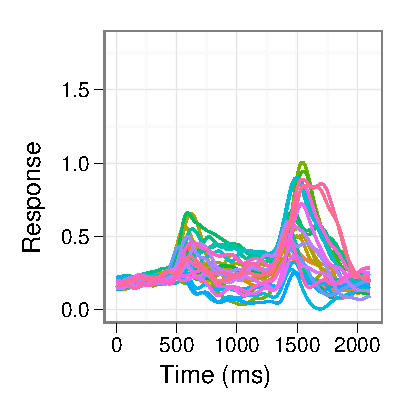
\includegraphics{neuron1}
        \end{center}
    \end{minipage}
    \begin{minipage}{0.61\textwidth}
        \begin{center}
            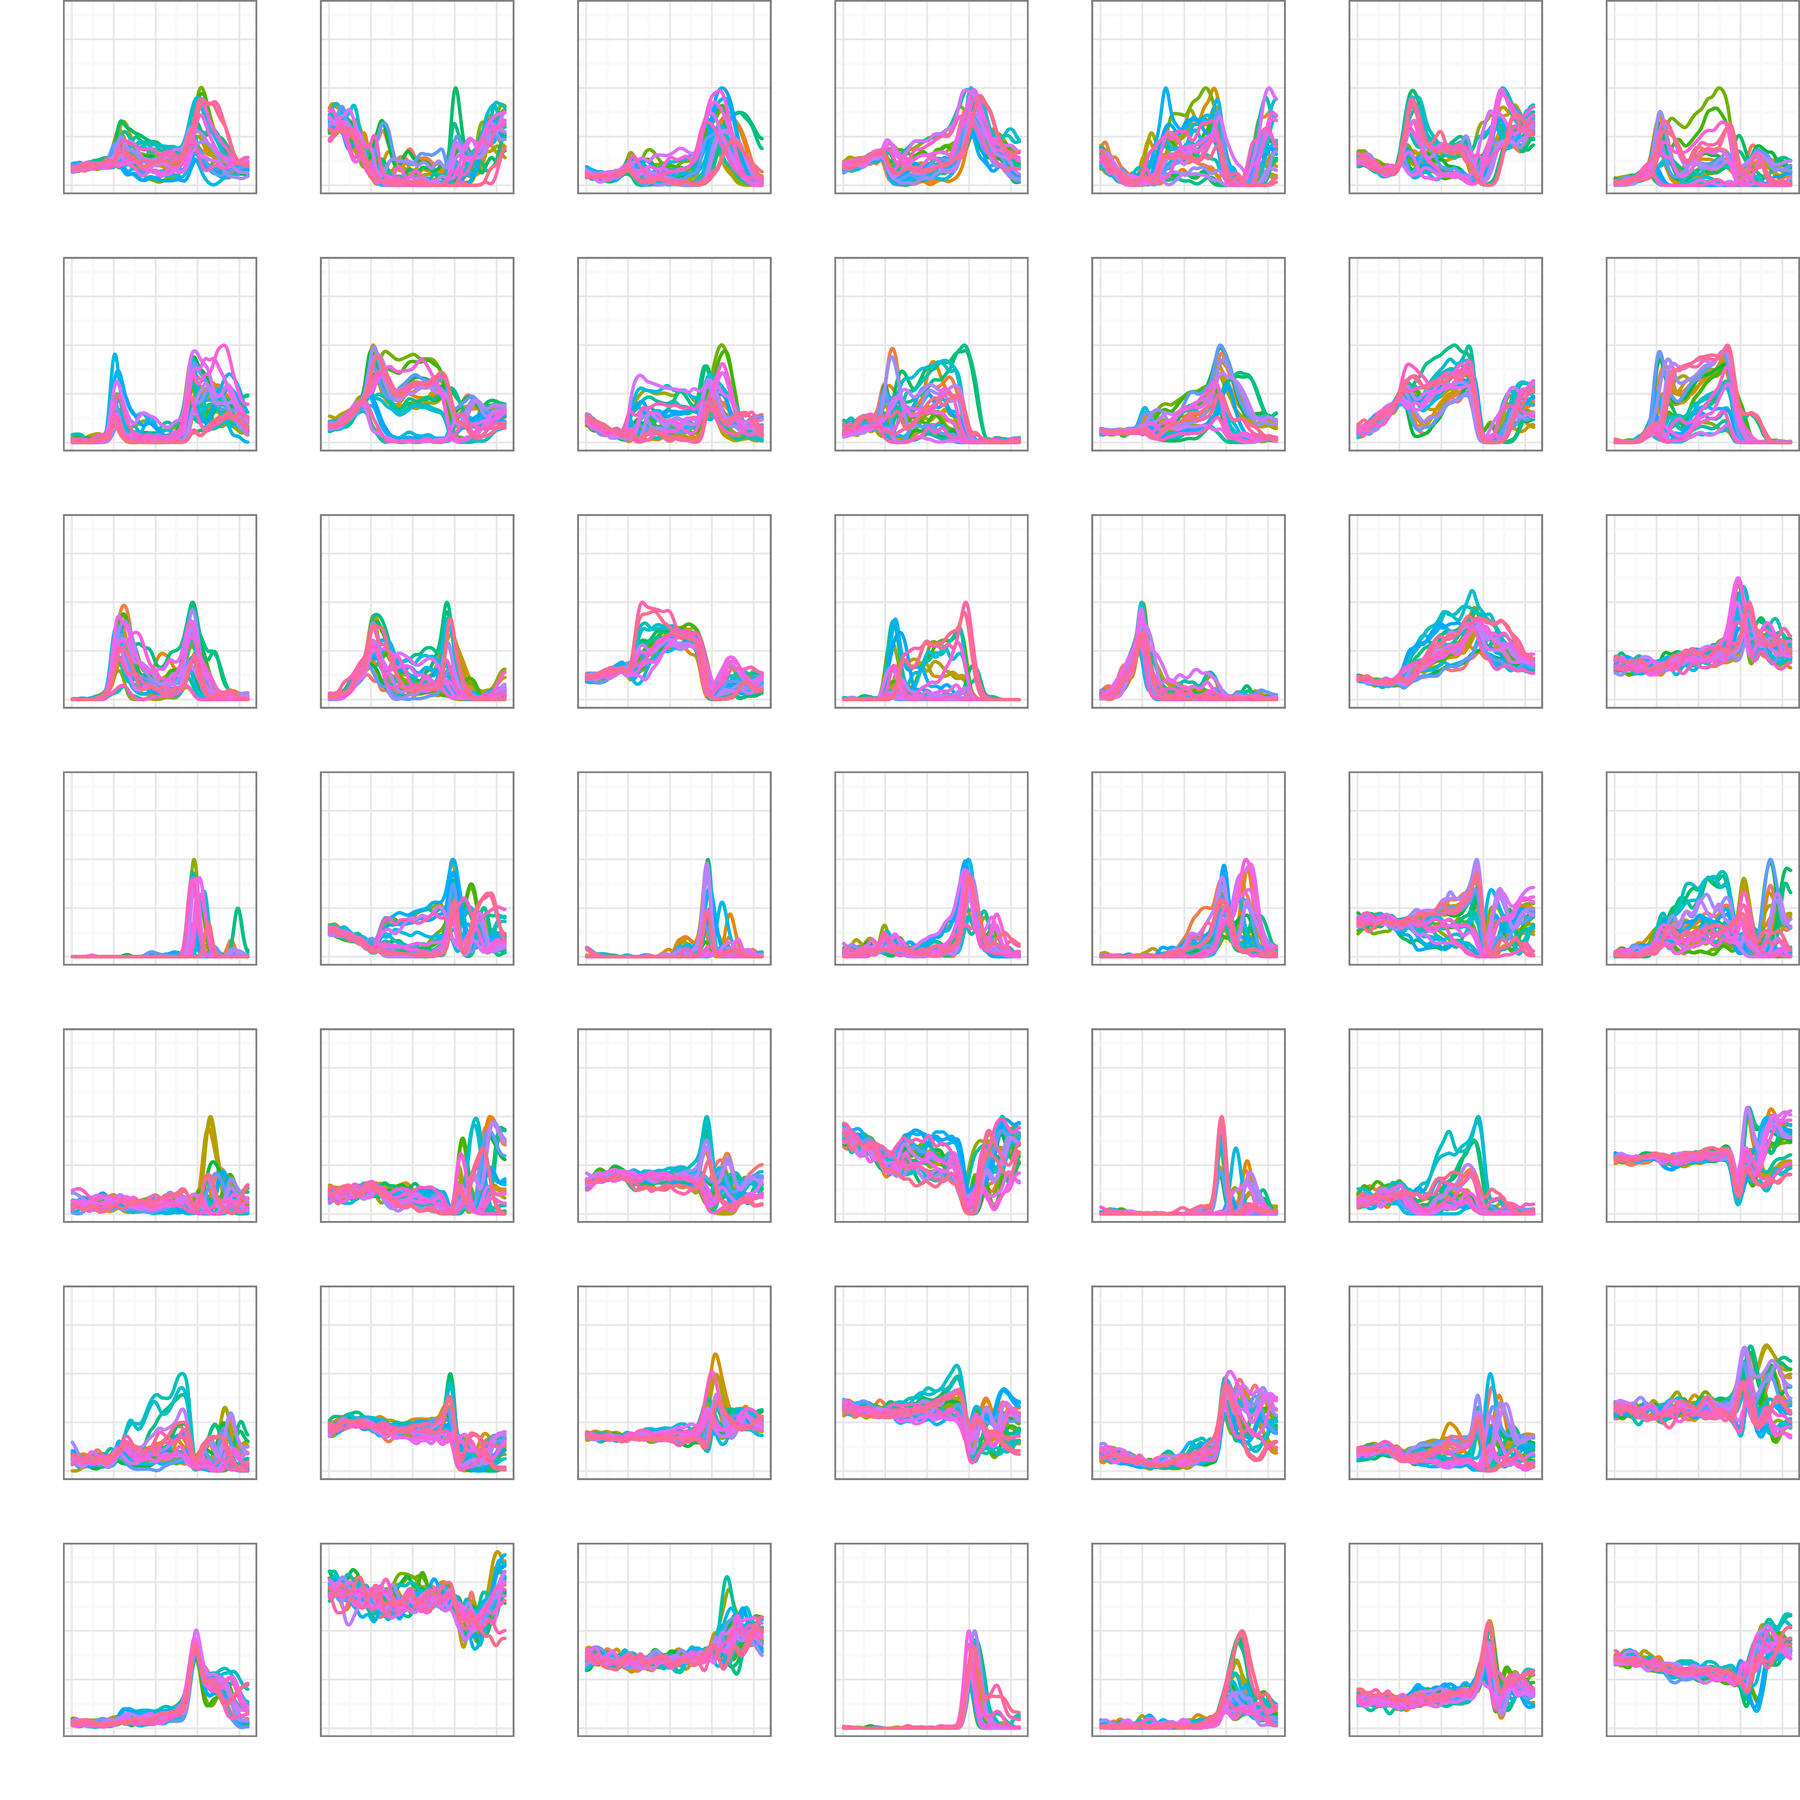
\includegraphics{neurons}
        \end{center}
    \end{minipage}
    \caption{
        \captiontitle{Motor cortex data}
        Response rates in 47 neurons for 27 movement tasks.  The subplots show
        the normalized response rates in a single neuron as functions of time.  
        Each color corresponds to a different movement task.  The plot on
        the left is a zoomed-in view of the data for the first neuron.
    }\label{F:motor-cortex-data}
\end{figure}

The data from the NSPL motor cortex experiment can be put into a matrix where
each neuron is thought of as a variable, and the timepoints of each condition
are thought of as observations. This gives us a matrix $\mX$ with $p = 49$
variables and $n = 27 \cdot 422 = 11394$ observations. Of course, the rows of
$\mX$ are nothing like \iid, and the noise in $\mX$ is not white. Parametric
methods are not likely to give very reliable estimates of the dimensionality
of $\mX$, but cross-validation stands a reasonable chance.

After centering the columns of $\mX$, we performed Wold- and Gabriel-style cross-validation to estimate the dimensionality of the signal part of $\mX$.  
For Gabriel-style CV, we first tried both $(2,2)$-fold and $(2,49)$-fold; both resulting $\widehat{PE}(k)$ curves had their minima at the maximum $k$.  For $5$-fold Wold-style CV, there is a minimum at $k=13$.  The BIC, $F$, MDL, and UIP estimators all chose $k=48$ as the dimensionality, while the AIC estimator chose $k=47$.  We show the cross-validation estimated prediction curves in Figure~\ref{F:motor-cv-est}

\begin{figure}
    \centering
    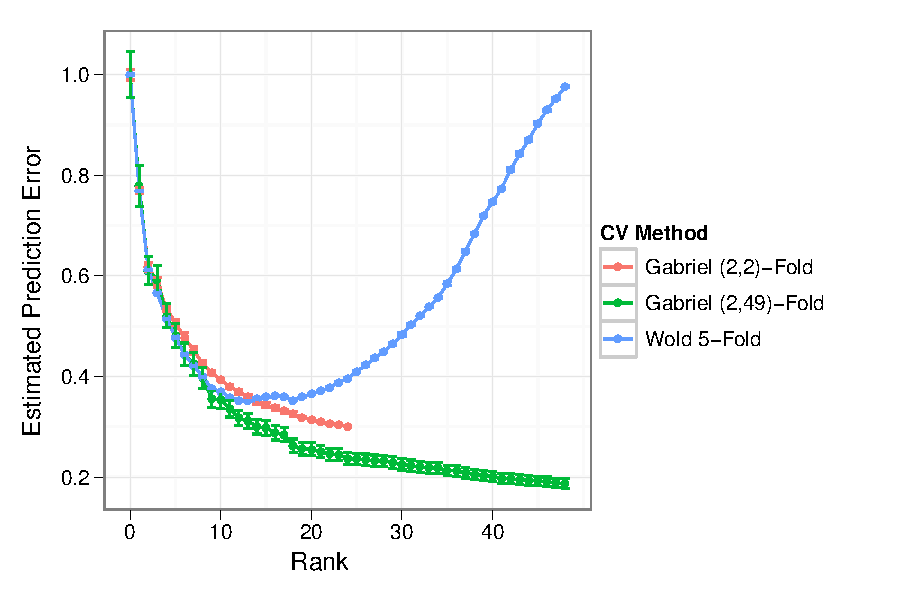
\includegraphics{motor-cv-est}
    \caption{
        \captiontitle{Motor cortex estimated prediction error}
        Prediction error as a function of rank, estimated by three 
        cross-validation methods.  The units are normalized so that the
        maximum prediction error is $1.0$.  Error bars show one standard    
        error, estimated from the folds. The prediction error estimate from
        Wold-style CV shows a minimum at $k=13$, but the Gabriel-style
        CV estimates always decrease with $k$.  
    }\label{F:motor-cv-est}
\end{figure}


\section{Summary and future work}

We have described two different forms of cross-validation appropriate for
model selection in unsupervised learning. Wold-style CV uses a ``speckled''
leav-out, and Gabriel-style CV uses a ``blocked'' leave-out. We have defined
two forms of error associated with SVD/PCA-like models, the prediction error
and the model error. Through simulaitons, we have shown that both forms of CV
can be considered to give estimates of prediction error. Both methods perform
well, but Wold-style CV seems to be more robust to badly-behaved noise. We
have applied these cross-validation methods to a data analysis problem from a
Neuroscience experiment.

We have focused on latent factor models and the singular value decomposition.
However, it is relatively easy to translate the two styles of cross-validation
presented here to other unsupervised learning methods. For Wold-style
hold-outs, an EM-like algorithm can usually be applied to the models in many
unsupervised learning contexts. The Gabriel-style philosophy of ``treat some
of the variables as response and the others as predictors'' can also be
applied more broadly. We are in the process of investigating both
cross-validation strategies for clustering and kernel-based manifold learning.

This chapter leaves a number of open questions.  Mainly, we have not provided 
any theoretical results here, only simulations.  A quote from Downton's 
discussion of Stone's 1974 paper on cross-validation equally applies to our 
work:
\begin{quote}
    A current nine-day wonder in the press concerns the exploits of a Mr. Uri
    Geller who appears to be able to bend metal objects without touching them;
    [The author] seems to be attempting to bend statistics without touching
    them. My attitude to both of these phenomena is one of open-minded 
    scepticism; I do not believe in either of these prestigious activities, on 
    the other hand they both deserve serious scientific examination
    \cite{stone1974cv}.
\end{quote}
Despite Dowton's skepticism, cross-validation has proven to be an invaluable tool for supervised learning.  It is our hope that with some additional work, CV can be just as valuable for unsupervised learning.  In the next chapter, we provide some theoretical justification for Gabriel-style cross-validation, but analysis of Wold-style cross-validation is still an open problem.

